%% XQdrant; EDBT 2027 short research paper
%% Official EDBT A4 / ACM sigconf skeleton (see edbt-macros.tex).
%% Compile:
%%   pdflatex main && bibtex main && pdflatex main && pdflatex main
%%
%% BEFORE SUBMISSION:
%%  - replace author / affiliation placeholders with real values
%%    (EDBT is single-anonymous: names MUST appear on the PDF)
%%  - confirm every author is registered on CMT
%%  - ensure title still starts with "[Short Paper]"
%%  - upload artifacts zip OR a no-access-monitoring repo link on CMT
%%  - keep body ≤ 6 pages; Artifacts + references are unlimited
%%  - no \pending{...} left:  grep -n 'pending{' main.tex

%% balance=false: acmart otherwise auto-\balance's the last page into two
%% short columns when only a few references overflow.
\documentclass[sigconf,review,balance=false]{acmart}

%% EDBT: A4 paper (official template override of letter-size defaults)
\geometry{twoside=true, head=13pt,
     a4paper,
     includeheadfoot, columnsep=2pc,
     top=57pt, bottom=73pt, inner=54pt, outer=54pt,
     marginparwidth=2pc,heightrounded
     }%

\AtBeginMaketitle{%
  %% EDBT Conference Proceedings setup for ACM sigconf Style



%% EDBT: ISBN and year have to be adapted with every Number / Volume !
%%
\def\EDBTISSN{xxxx-xxxx}
\def\EDBTISBN{xxx-x-xxxxx-xxx-x}
\setcopyright{none}
\copyrightyear{\copyright\ 2027 Copyright held by the owner/author(s).
  Published on xxxxx under ISBN \EDBTISBN, series ISSN \EDBTISSN.
  Distribution of this paper is permitted under the terms of the
  Creative Commons license CC-by-nc-nd 4.0}
\acmYear{2027}
\acmDOI{}
\acmISBN{}


%% These commands are for a PROCEEDINGS abstract or paper.
%% EDBT: This needs adaptation every year!
\acmConference[EDBT '27]{Extending Database Technology}{6-9 April 2027}{Lille (France)}
%%
%%  Uncomment \acmBooktitle if the title of the proceedings is different
%%  from ``Proceedings of ...''!
%%
%%\acmBooktitle{Woodstock '18: ACM Symposium on Neural Gaze Detection,
%%  June 03--05, 2018, Woodstock, NY}


%% EDBT:
\settopmatter{printacmref=false, printccs=false, printfolios=false}


%% EDBT:
%% Macro to make image usable as hyperlink [see http://tex.stackexchange.com/questions/31819/xelatex-includegraphics-and-hyperlink]
\newsavebox{\ximagebox}
\newlength{\ximageheight}
\newsavebox{\xglyphbox}
\newlength{\xglyphheight}
\newcommand{\xbox}[1]%
  {\savebox{\ximagebox}{#1}%
  \settoheight{\ximageheight}{\usebox{\ximagebox}}%
  \savebox{\xglyphbox}{\color{white}\char32}%
  \settoheight{\xglyphheight}{\usebox{\xglyphbox}}%
  \raisebox{\ximageheight}[0pt][0pt]{\raisebox{-\xglyphheight}[0pt][0pt]{%
    \makebox[0pt][l]{\usebox{\xglyphbox}}}}%
    \usebox{\ximagebox}%
    \raisebox{0pt}[0pt][0pt]{\makebox[0pt][r]{\usebox{\xglyphbox}}}}

%% now use this to define the logo header:

\newsavebox{\LogoBox}
\sbox{\LogoBox}{}

%% now define our header and footer for the first page
\fancypagestyle{firstpagestyle}{%
  \fancyhf{}%
  \fancyfoot{}%
  \fancyhead[L,C]{}
  \fancyhead[R]{}{\raisebox{15pt}[0pt][0pt]{\xbox{\usebox{\LogoBox}}}}
  }

\hypersetup{%
  pdfcopyright={CC-by-nc-nd},
  pdfcreator={LaTeX with acmart, hyperref, and EDBT modifications},
  pdfvolumenum={XX},
  pdfissuenum={X},
  pdfisbn={\EDBTISBN},
  pdfissn={\EDBTISSN}
}

}% \AtBeginMaketitle

\usepackage{graphicx}
\usepackage{array}
\usepackage{xcolor}
\graphicspath{{figures/}}

%% Allow breaks after \_ so long identifiers wrap in-column.
\newcommand{\breakablecode}[1]{%
  {\ttfamily
    \renewcommand{\_}{\textunderscore\allowbreak}%
    #1%
  }}

%% Values still to be filled in by the author (rendered red).
\newcommand{\pending}[1]{\textcolor{red}{#1}}

\begin{document}

%% EDBT short-paper rule: title MUST start with "[Short Paper]"
\title{[Short Paper] Which Neighbors Count? Query-Time Subspace Search
  and In-Database Attribution in XQdrant}

%% EDBT is single-anonymous: include real names/affiliations before submit.
\author{Moetez Fradi}
\email{moetez.fradi@insat.ucar.tn}
\affiliation{%
  \institution{INSAT}
  \city{Tunis}
  \country{Tunisia}
}

\renewcommand{\shortauthors}{Fradi}

\begin{abstract}
Vector databases return opaque scalar similarities over high-dimensional
embeddings, giving practitioners no coordinate-level explanation of a match and
no way to restrict HNSW traversal itself to a dynamic focus subspace. We present
\textbf{XQdrant}, an extension of the Qdrant engine that addresses both.

\emph{Attribution}: \texttt{with\_dims\_explained} computes exact top-$m$
per-dimension score decomposition in-database, avoiding client-side vector
egress. It leaves the ranked result unchanged, adds about 0.4\,ms of in-engine
time independent of $m$, and runs $\sim$1.8$\times$ faster end to end than
post-query extraction at encoder-scale widths ($D\in\{768,1536\}$).

\emph{Masked-distance HNSW traversal} scores only the focus subspace during
descent over an unmodified full-space graph, and evaluating it requires two
ground truths. Against full-space ground truth, masked search on SIFT1M scores
exactly the subspace/full-space $k$-NN \emph{coherence} ($0.012$ vs.\ $0.013$
at $D_{\mathrm{sub}}/D=0.1$), a property of the data rather than a navigation
failure. Against subspace ground truth, it finds the focus-metric neighbors
with Recall@10 of at least $0.91$ when the focus set covers half the dimensions
or more, but $0.77$ at a quarter and about $0.4$ at a tenth; keeping
full-distance routing on the upper layers (\texttt{mask\_from\_layer}) changes
this by at most $0.04$. In-engine, masked search runs at $0.70$--$0.89\times$
the speed of plain search: with every dimension in focus it returns identical
results yet takes $1.6\times$ as long, so the per-distance cost of
non-contiguous scoring, not traversal, rules out a latency win. Overfetch plus
full-distance verification recovers full-space recall where coherence allows
($0.48\rightarrow 0.91$ at $D_{\mathrm{sub}}/D=0.75$) for under 0.3\,ms, and an
$\alpha$-weighted full/masked blend never improves on pure masking. We release
the harness and an experiment index that maps each claim to a script.
\end{abstract}

\begin{CCSXML}
<ccs2012>
   <concept>
       <concept_id>10002951.10002952.10003190.10010509</concept_id>
       <concept_desc>Information systems~Nearest-neighbor search</concept_desc>
       <concept_significance>500</concept_significance>
   </concept>
   <concept>
       <concept_id>10002951.10002952.10003190</concept_id>
       <concept_desc>Information systems~Database query processing</concept_desc>
       <concept_significance>400</concept_significance>
   </concept>
</ccs2012>
\end{CCSXML}

\ccsdesc[500]{Information systems~Nearest-neighbor search}
\ccsdesc[400]{Information systems~Database query processing}

\keywords{vector databases, HNSW, approximate nearest neighbor,
  explainability, feature attribution, subspace search, masked distance, SIMD}

\maketitle

%=============================================================================
\section{Introduction}
\label{sec:intro}

High-dimensional dense embeddings underpin retrieval-augmented generation
(RAG), recommendation, and semantic search~\cite{lewis2020rag,qdrant2024,wang2021milvus}.
Production engines traverse HNSW graphs~\cite{malkov2018hnsw}, collapsing every
comparison into a single scalar. This creates two gaps that motivate this paper.

\textbf{Explainability.} Practitioners cannot see which coordinates drove a hit
without fetching full vectors and recomputing per-dimension terms client-side,
an expensive, egress-bound pattern.

\textbf{Subspace routing.} Many workloads care about a dynamic focus set
$\mathcal{F}$ of coordinates (concept probes, ablations, modality masks), yet
stock HNSW always evaluates full $D$-dimensional distances during graph descent.
Rescoring on $\mathcal{F}$ after full-vector preselection improves semantic
specificity but, as we show, cannot reduce traversal cost.

\textbf{XQdrant} addresses the first gap and characterizes the second. For
attribution, \texttt{with\_dims\_explained} attaches exact top-$m$ coordinate
terms to search results in-database. For subspace routing,
\texttt{nearest.focus} with \texttt{masked=true} evaluates reduced distances
\emph{during} HNSW traversal, not just after it, with a hybrid layer cutoff,
gather-based SIMD kernels, an optional verify/overfetch pass, and a
full/masked score blend. Evaluating masked traversal requires care about which
neighbors count as correct. Recall against full-space ground truth measures
whether two metrics agree; recall against subspace ground truth measures
whether traversal navigates. Keeping the two apart changes the conclusions
(Section~\ref{sec:eval-gt}).

\subsection*{Contributions}
\vspace{-0.35em}
\begin{itemize}
  \setlength{\itemsep}{0.2em}
  \setlength{\parsep}{0pt}
  \setlength{\topsep}{0.15em}
  \setlength{\partopsep}{0pt}
  \item \textbf{In-database attribution.} Exact score decomposition with
    order-statistic top-$m$ selection; about 0.4\,ms in-engine and
    $\sim$1.8$\times$ faster than post-query extraction, with the ranked
    result unchanged.
  \item \textbf{Masked-distance HNSW traversal, evaluated under two ground
    truths.} On SIFT1M it navigates well for large focus sets and degrades
    for small ones, a layer cutoff barely changes this, and it never beats
    plain search; we trace the latency gap to per-distance cost.
  \item \textbf{Coherence as the reference for full-space recall.}
    Subspace/full-space $k$-NN overlap matches the full-space recall of
    masked search and predicts when a verify pass can recover full-space
    neighbors, independent of the traversal strategy.
  \item \textbf{Reproducible artifacts.} A public experiment index and harness
    (Section~\ref{sec:artifacts}) mapping every claim above to a canonical
    script and dataset.
\end{itemize}

%=============================================================================
\section{Background}
\label{sec:background}

\subsection{HNSW and Contiguous SIMD}

HNSW maintains multi-layer proximity graphs~\cite{malkov2018hnsw}. Queries
greedily descend with candidate heap size \texttt{ef\_search}, then extract
top-$k$ at the base layer. Distance kernels assume contiguous \texttt{f32}
slices (AVX2/NEON), so a non-contiguous focus set must either (i) repack
selected coordinates into a scratch buffer before scoring, or (ii) gather them
directly via SIMD gather loads.

\subsection{Score Decomposition}

For Dot product, $s(\mathbf{q},\mathbf{v})=\sum_i q_i v_i$; Cosine applies the
same decomposition after $\ell_2$ normalization; Euclidean and Manhattan admit
analogous additive terms. Attribution is therefore exact accounting of the
engine's own metric, not an estimate (Section~\ref{sec:related}).

\subsection{Subspace Coherence}
\label{sec:coherence-def}

Let $N_k^{\mathrm{full}}(q)$ and $N_k^{\mathcal{F}}(q)$ denote exact $k$-NN sets
under the full metric and under focus set $\mathcal{F}$. We define
\emph{coherence} as $|N_k^{\mathrm{full}}\cap N_k^{\mathcal{F}}|/k$ and call
this diagnostic \textbf{C1}. Coherence is the full-space Recall@$k$ that an
\emph{exact} subspace search achieves; it depends on the data and
$\mathcal{F}$, not on any index. Masked traversal thus has two accuracy
measures. \emph{Subspace recall}, against $N_k^{\mathcal{F}}$, asks whether
traversal found the focus-metric neighbors, i.e., whether the graph remains
navigable. \emph{Full-space recall}, against $N_k^{\mathrm{full}}$, asks
whether those neighbors are also full-space neighbors; for a search that
returns $N_k^{\mathcal{F}}$ exactly, it equals coherence.

%=============================================================================
\section{In-Database Attribution}
\label{sec:attribution}

XQdrant injects attribution at the collection coordinator after shard merge,
with an early return when \texttt{with\_dims\_explained} is absent, so other
requests take the unmodified path. Per explained hit, Algorithm~\ref{alg:attribution}
materializes $D$ terms and selects the top-$m$ by absolute contribution in
average $\mathcal{O}(D)$ time via Rust's order-statistic selection
(\breakablecode{select\_nth\_unstable}).

\begin{figure}[htbp]
\centering
\begin{minipage}{0.92\linewidth}
\small
\textbf{Algorithm 1} (In-database top-$m$ attribution).\\
\textbf{Input:} query $\mathbf{q}$, vector $\mathbf{v}$, $D$, $m$, metric $\delta$.\\
1.\ Normalize operands if required by $\delta$.\\
2.\ For $i=0,\ldots,D-1$: append $(i,\textsc{Term}_i(\mathbf{q},\mathbf{v},\delta))$.\\
3.\ Return order-statistic top-$m$ by $|t|$, sorted descending.
\end{minipage}
\caption{In-database top-$m$ feature attribution.}
\label{alg:attribution}
\end{figure}

\texttt{nearest.focus} without masking still performs full HNSW preselection
and rescores on $\mathcal{F}$ afterward, useful when ranking must respect a
focus subspace, but, as Section~\ref{sec:eval-attr} shows, not a
traversal-cost reduction. That gap is exactly what motivates masked
traversal (Section~\ref{sec:masked}).

%=============================================================================
\section{Masked-Distance HNSW: Design Space}
\label{sec:masked}

We consider three traversal-level strategies for evaluating distance only over
a focus subspace $\mathcal{F}$ during HNSW descent, plus two supporting
mechanisms (a kernel choice and a recall-recovery pass) that apply across all
three. Table~\ref{tab:namemap} fixes the naming used for the rest of the paper.

\begin{table}[htbp]
  \centering
  \caption{Naming used throughout Sections~\ref{sec:masked}--\ref{sec:eval}.}
  \label{tab:namemap}
  \small
  \begin{tabular}{|l|p{5.4cm}|}
    \hline
    \textbf{Name} & \textbf{What it is} \\
    \hline
    M1 & Naive: mask every HNSW layer \\
    M2 & Hybrid: full distance for layers $\geq L$, masked below (\breakablecode{mask\_from\_layer}$=L$) \\
    M3 & M2 plus an $\alpha$-weighted blend of full/masked scores on masked layers \\
    \hline
    K1 & Kernel choice: repack-then-score vs.\ SIMD gather, orthogonal to M1--M3 \\
    V1 & Verify/overfetch: optional post-traversal full-distance rescore, orthogonal to M1--M3 \\
    C1 & Coherence diagnostic (Section~\ref{sec:coherence-def}), used to interpret M1--M3 and V1 \\
    \hline
  \end{tabular}
\end{table}

\subsection{API Surface}

Focus parameters ride inside the existing query body:
\begin{verbatim}
"focus": {
  "dims": [...], "masked": true,
  "mask_from_layer": 1,   // M2/M3 hybrid cutoff
  "verify": true,         // optional full rescore
  "alpha": 0.25           // M3 blend weight
}
\end{verbatim}
Constraints mirror existing dense local-search paths: no quantization/turbo, no
simultaneous \texttt{with\_dims\_explained} on masked paths, and fail-fast if
\texttt{mask\_from\_layer}, \texttt{verify}, or \texttt{alpha} are set without
\texttt{masked=true}.

\subsection{M1: Naive All-Layer Masking}

With \texttt{masked=true} and no cutoff, every HNSW comparison during descent
uses only coordinates in $\mathcal{F}$. This is the simplest semantic change
and the natural first attempt. The concern is navigability: graph edges encode
full-space proximity, so greedy descent under a different metric has no
guarantee of reaching the focus-metric neighbors. Section~\ref{sec:eval-gt}
tests this directly.

\subsection{M2: Hybrid Layer Cutoff}

M2 keeps full-distance routing where the graph is coarsest and masks only near
the base layer, where the final candidates are chosen. Layer $\ell$ uses the
masked scorer iff $\ell < L$ for cutoff
$L ={}$\breakablecode{mask\_from\_layer}; otherwise full distance is used.
$L{=}0$ recovers plain (unmasked) nearest search; a large $L$ recovers M1.
The implementation builds dual raw scorers inside \texttt{FilteredScorer}
and switches via \texttt{set\_layer} at layer boundaries; visited-set and
heap logic are unchanged, so this composes with the rest of the query
pipeline for free.

\subsection{M3: Weighted Blend}

On masked layers, score $= \alpha \cdot s_{\mathrm{full}} + (1-\alpha)\cdot
s_{\mathrm{focus}}$; coarse (unmasked) layers are unaffected. Note that
blending computes \emph{both} distances, so it cannot reduce arithmetic cost on
its own; it exists purely as a routing-bias ablation to test whether it
recovers recall at a fixed cutoff more cheaply than raising $L$.

\subsection{K1: Kernel Choice: Repack vs.\ Gather}

Masked scoring can copy focus dims into a contiguous scratch buffer before
calling the existing SIMD kernels (\emph{repack}), or gather them directly
in-register (AVX2 gather for Dot/Cosine/Euclidean on x86; scalar fallback
elsewhere). We add the gather path, selectable via environment variable
\breakablecode{XQDRANT\_MASKED\_KERNEL}, and treat kernel choice as
orthogonal to M1--M3: any of the three can use either kernel.

\subsection{V1: Verify and Overfetch}

\texttt{verify=true} re-scores returned candidates with full distance after
traversal, reusing the existing quantization-rescore hook. At overfetch
$m{=}1$ (i.e., $\mathit{limit}=k$) this only reorders a size-$k$ set, so
Recall@$k$ is provably unchanged; it is a correctness/ordering feature, not a
recall-recovery one. Overfetch with $m>1$ ($\mathit{limit}=m\cdot k$, keep
top-$k$ after full rescore) turns masked traversal into a candidate
\emph{filter} and can recover recall, at a latency cost we quantify in
Section~\ref{sec:eval-verify}.

%=============================================================================
\section{Experimental Evaluation}
\label{sec:eval}

Table~\ref{tab:keep} at the end of this section summarizes the verdict for
each mechanism.

\subsection{Setup}

\paragraph{Hosts and protocol.} Host~A (\pending{CPU model, cores, RAM},
Linux) runs the attribution suite against vanilla Qdrant (1.18.3-dev, commit
\texttt{b4e9326}) and the kernel microbenchmarks. Host~B (AMD Ryzen~5~220,
6~cores/12~threads, 15\,GB RAM) runs every masked-traversal experiment and all
in-engine timings, with XQdrant at commit \texttt{ed5ca79} (opt-level~3, no
LTO) in WSL2 Ubuntu~24.04; its plain-search baseline is XQdrant without focus
parameters, which takes the unmodified Qdrant path. Collections use HNSW with
$M{=}16$ and \texttt{ef\_construct}${=}200$, no quantization, and, unless
swept, \texttt{ef}${=}128$; the masked kernel is gather unless the kernel is
the subject. All masked-traversal comparisons on a corpus share one index, so
differences between mechanisms are not confounded by index construction.
Unless a caption says otherwise, each configuration is the mean of $T{=}5$
trials with distinct seeds that redraw the focus set and, where applicable,
the query sample, with sample standard deviation as error bars. A focus set at
ratio $r$ is a uniformly random subset of $\mathrm{round}(rD)$ coordinates.
In-engine latency is Qdrant's server-side request time, which excludes HTTP
and serialization; client round trips over keep-alive connections can add a
${\sim}40$\,ms TCP delayed-ACK stall for multi-packet messages, which would
swamp the sub-millisecond effects we measure.

\paragraph{Attribution suite.} Synthetic corpora with $N{=}10\mathrm{k}$
vectors and $Q{=}500$ queries at $D\in\{768,1536\}$; baselines are vanilla
Qdrant and post-query extraction, which fetches the result vectors
(\breakablecode{with\_vector}) and computes the top-$m$ terms in the client.

\paragraph{Masked-traversal suite.} SIFT1M~\cite{jegou2011pq} ($D{=}128$,
Euclidean, $N{=}1\mathrm{M}$, $Q{=}500$, $k{=}10$), on which plain HNSW
search reaches Recall@10 of $0.99$, and a synthetic corpus with
$N{=}50\mathrm{k}$ at $D{=}768$: i.i.d.\ standard-normal vectors,
$\ell_2$-normalized, scored by Dot product.

\subsection{Attribution and Focus Rescoring Are Not the Same Problem}
\label{sec:eval-attr}

Attribution annotates an already-ranked result, so it cannot change recall:
at $D{=}768$, Recall@10 is identical for vanilla Qdrant and for XQdrant with
$m{=}10$ attributions at every \texttt{ef} we tested. In-engine (host~B), it
adds $0.36$--$0.40$\,ms to a $2.45$\,ms plain search, about 15\%, and the
cost barely depends on $m$ ($2.81$, $2.81$, and $2.85$\,ms for $m=1$, $10$,
$50$). The relevant comparison is post-query extraction, the only
alternative available to a client: Figure~\ref{fig:attribution-depth} shows
in-database attribution holds a flat mean p50 of $3.85$--$4.02$\,ms
($\pm\!0.07$) across $m\in\{1,\ldots,50\}$ while post-query extraction sits at
$6.87$--$7.03$\,ms ($\approx 1.78\times$). Figure~\ref{fig:subspace-rescore}
shows that \texttt{nearest.focus} \emph{rescoring}, which reuses full-vector
preselection, yields speedup $<1$ ($0.80$--$0.84$; $0.80$ in-engine on
SIFT1M): it reduces the dimensionality of the arithmetic but not the
traversal it depends on. This motivates masking the traversal itself.

\begin{figure}[htbp]
  \centering
  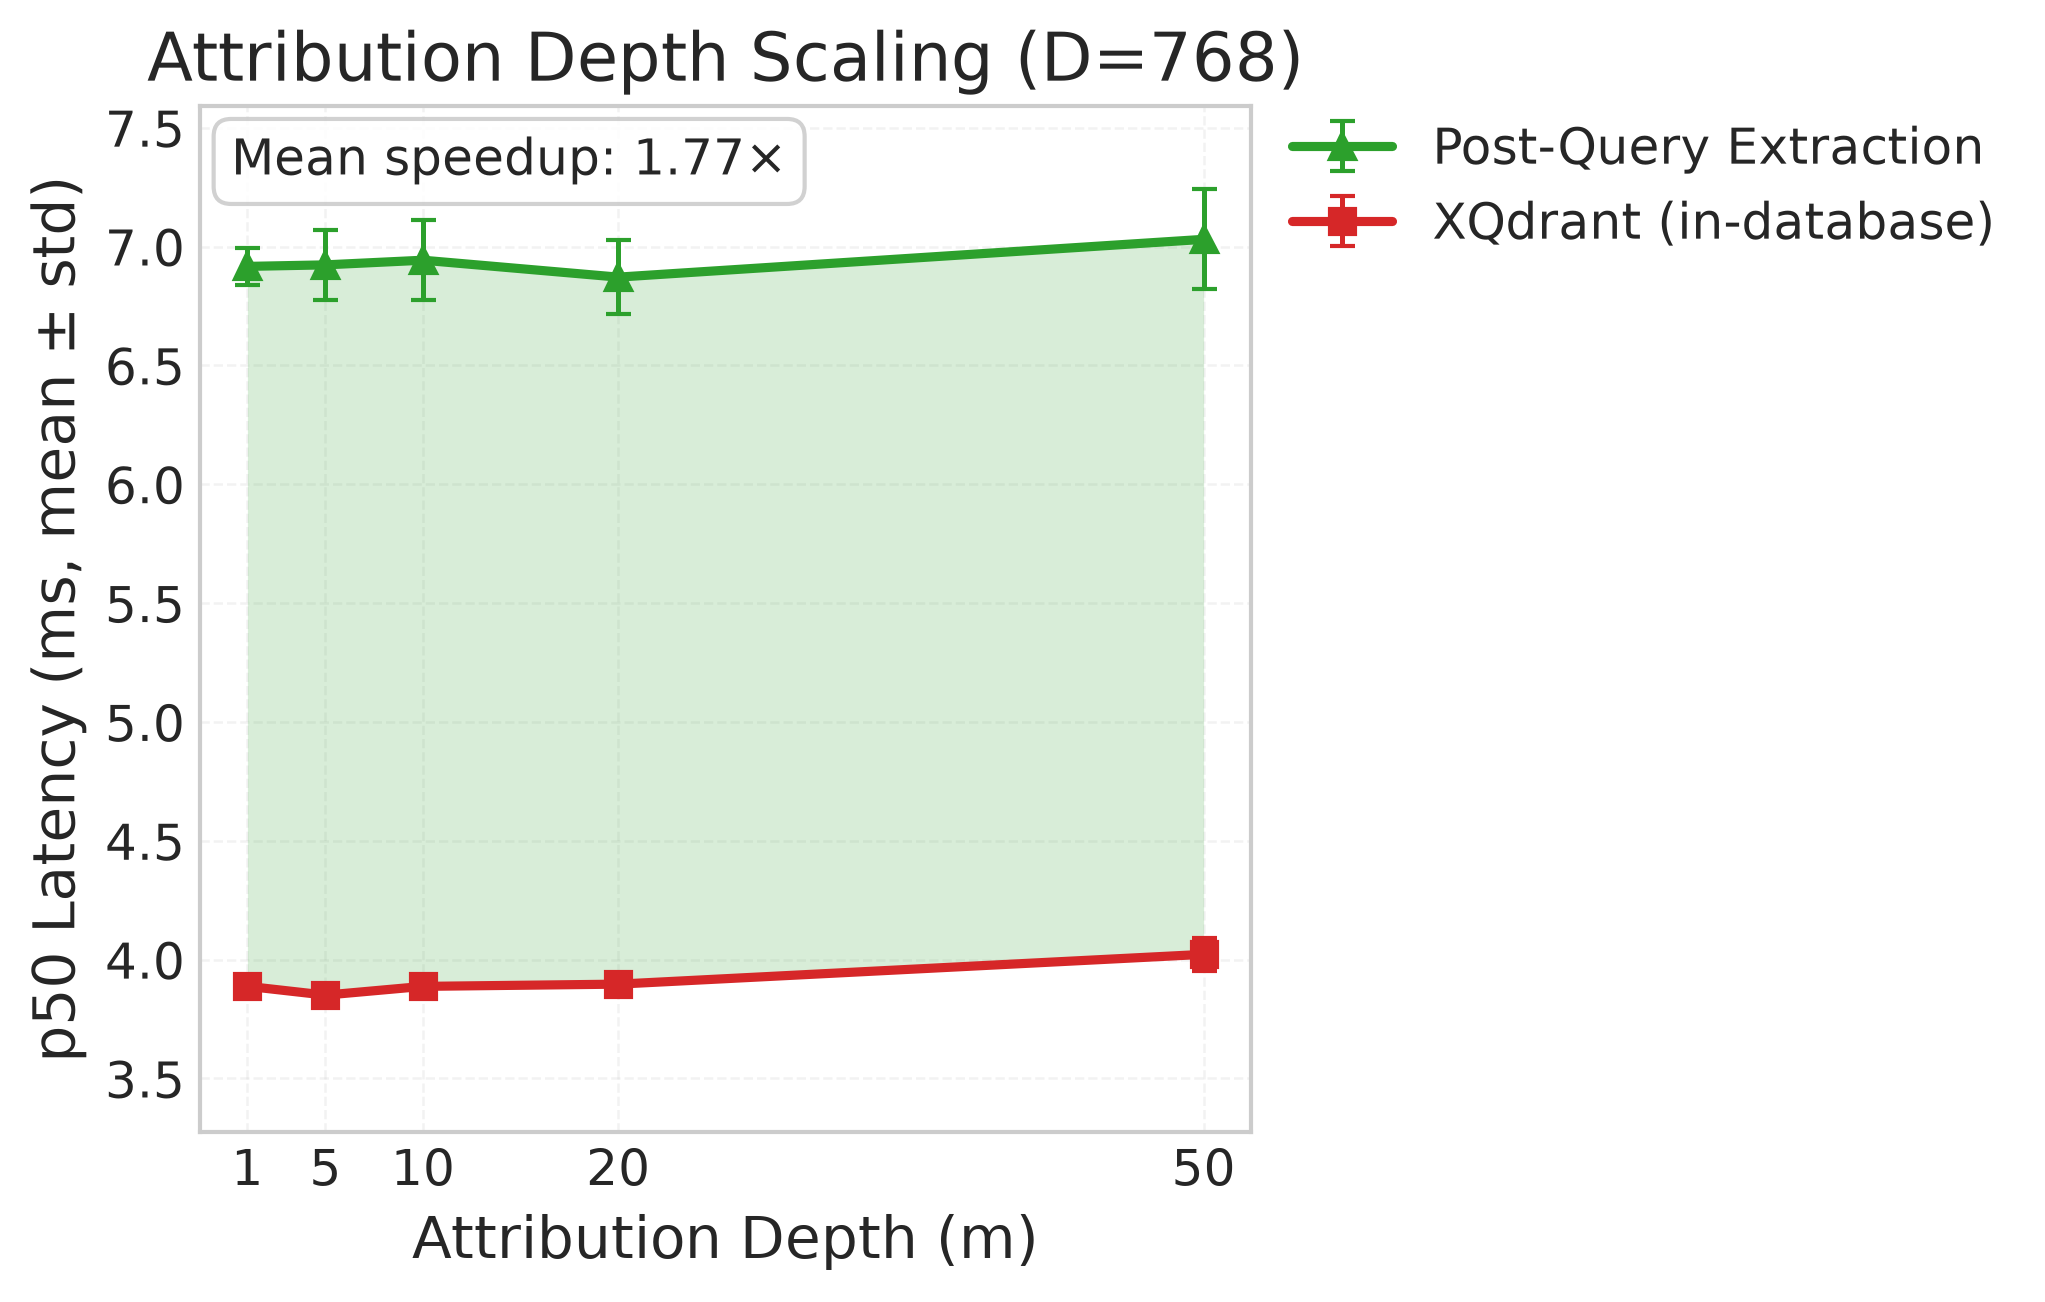
\includegraphics[width=0.92\linewidth]{plot3_attribution_depth_d768.png}
  \caption{Attribution depth: in-DB vs.\ post-query extraction ($D{=}768$,
    host~A, client-observed). Mean$\pm$std over $T{=}5$ trials.}
  \label{fig:attribution-depth}
\end{figure}

\begin{figure}[htbp]
  \centering
  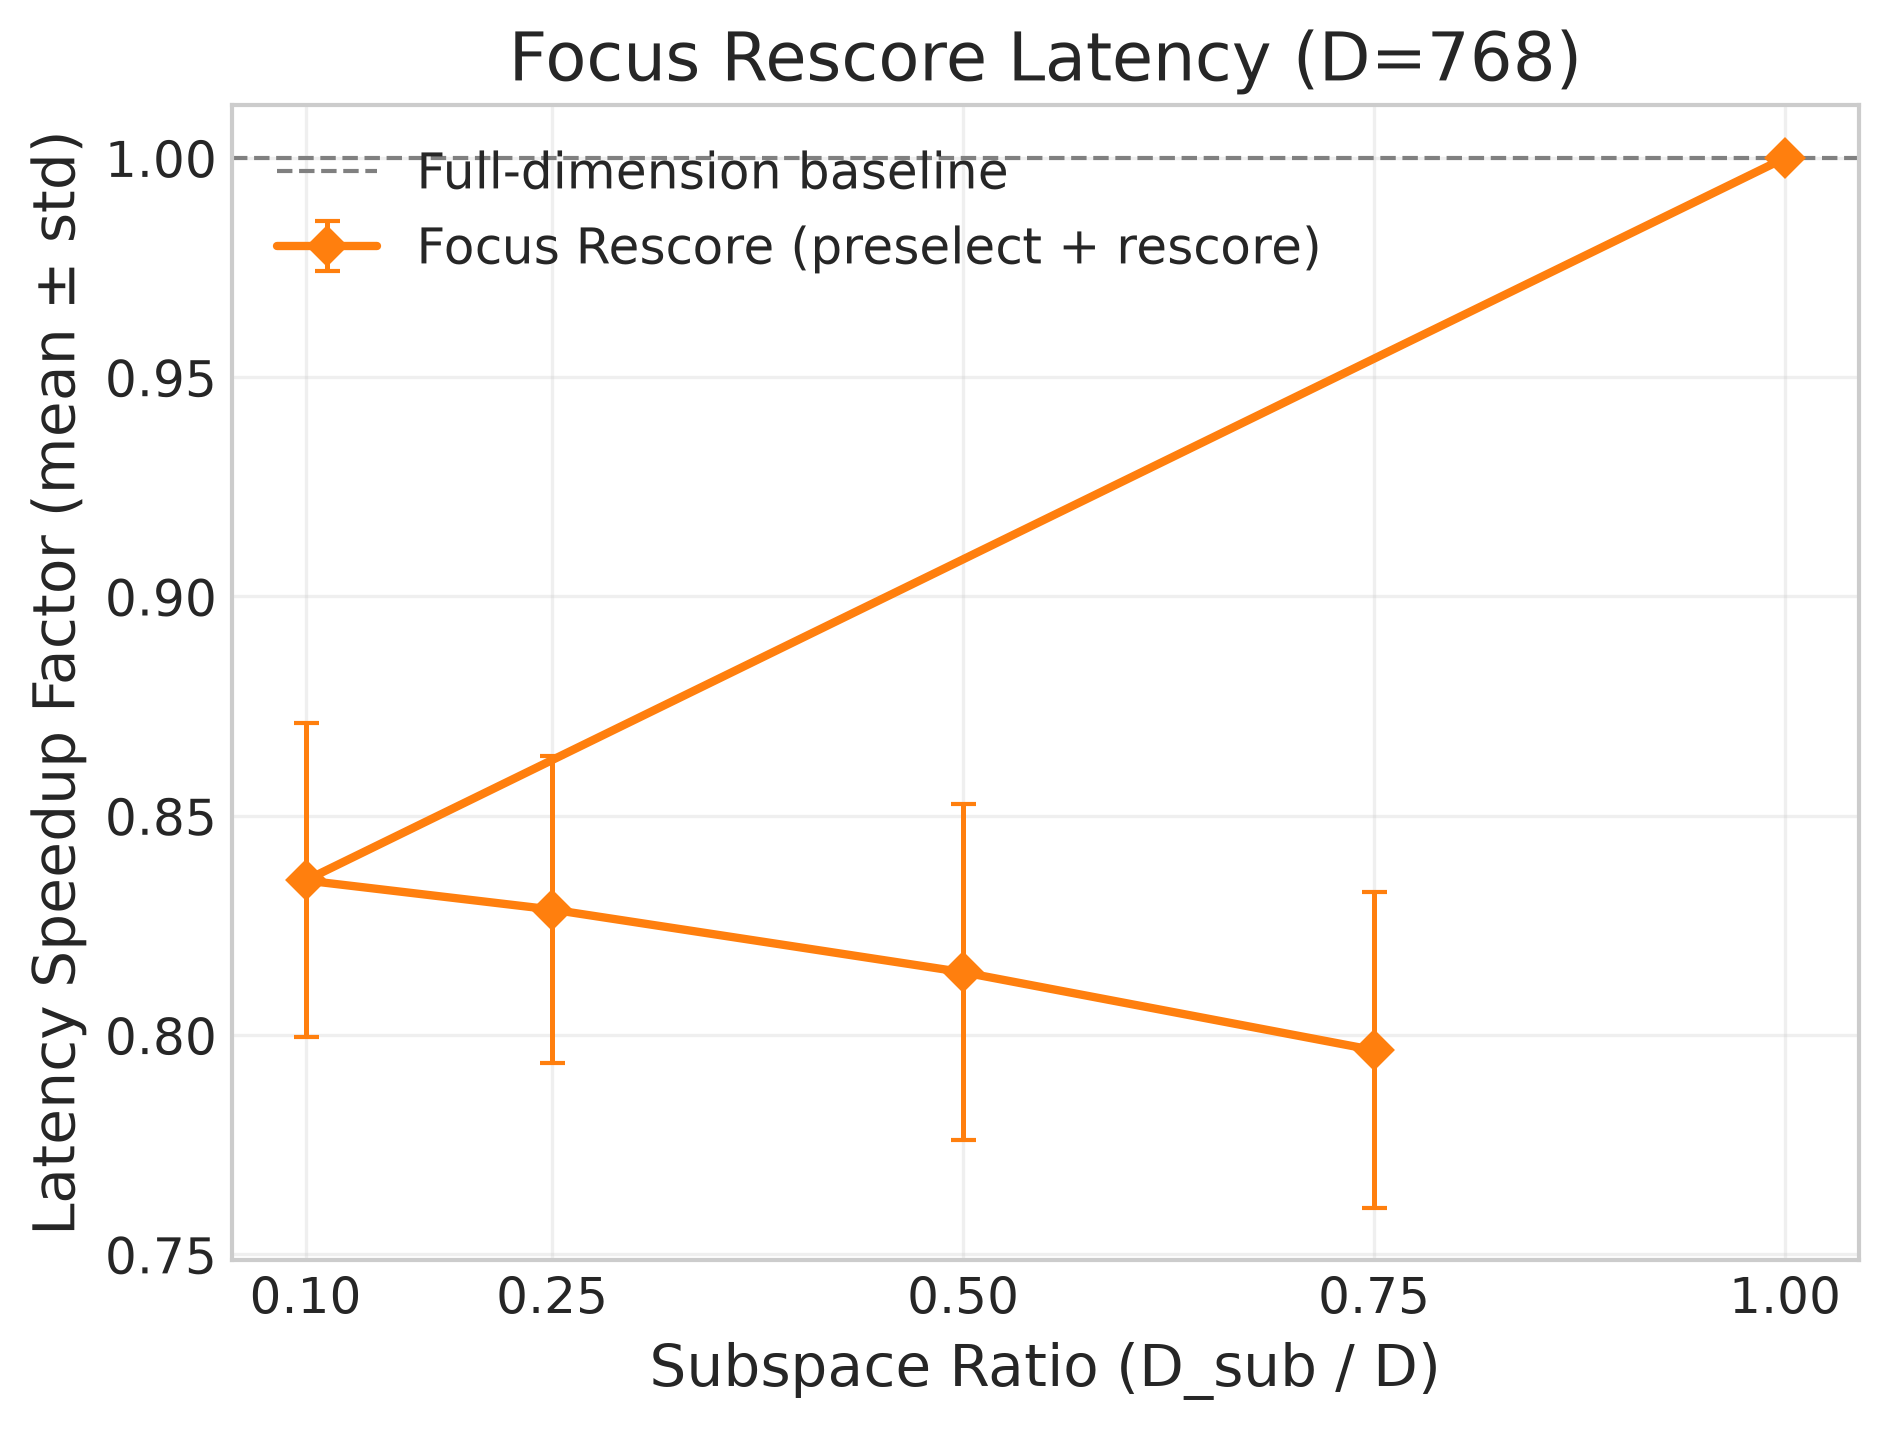
\includegraphics[width=0.92\linewidth]{plot4_subspace_speedup_d768.png}
  \caption{Focus \emph{rescoring} speedup $T_{\mathrm{full}}/T_{\mathrm{sub}}$
    ($D{=}768$, host~A): values $<1$ show rescoring alone does not
    accelerate search (mean$\pm$std, $T{=}5$).}
  \label{fig:subspace-rescore}
\end{figure}

\subsection{M1 and C1: Two Questions, Two Ground Truths}
\label{sec:eval-gt}

If rescoring cannot help, the next step is to mask distance \emph{during}
traversal (M1). Figure~\ref{fig:m1} evaluates M1 on SIFT1M against both
ground truths, together with exact coherence. Against full-space ground
truth, Recall@10 falls from $0.99$ at ratio $1.0$ to $0.490$, $0.253$,
$0.078$, and $0.012$ at ratios $0.75$, $0.5$, $0.25$, and $0.1$; read alone,
this looks like a navigability collapse. But coherence, computed without any
index, matches it at every ratio ($0.490$, $0.250$, $0.075$, $0.013$): M1
scores what a correct subspace search would, and the full-space numbers
measure disagreement between the two metrics, not a failure to navigate.
Against subspace ground truth, M1 finds the focus-metric neighbors with
Recall@10 of $0.98$ and $0.93$ at ratios $0.75$ and $0.5$, but only $0.77$ at
$0.25$ and $0.38$ at $0.1$. Navigability therefore holds for large focus sets
and degrades for small ones, a much milder effect than the full-space numbers
suggest.

\begin{figure}[htbp]
  \centering
  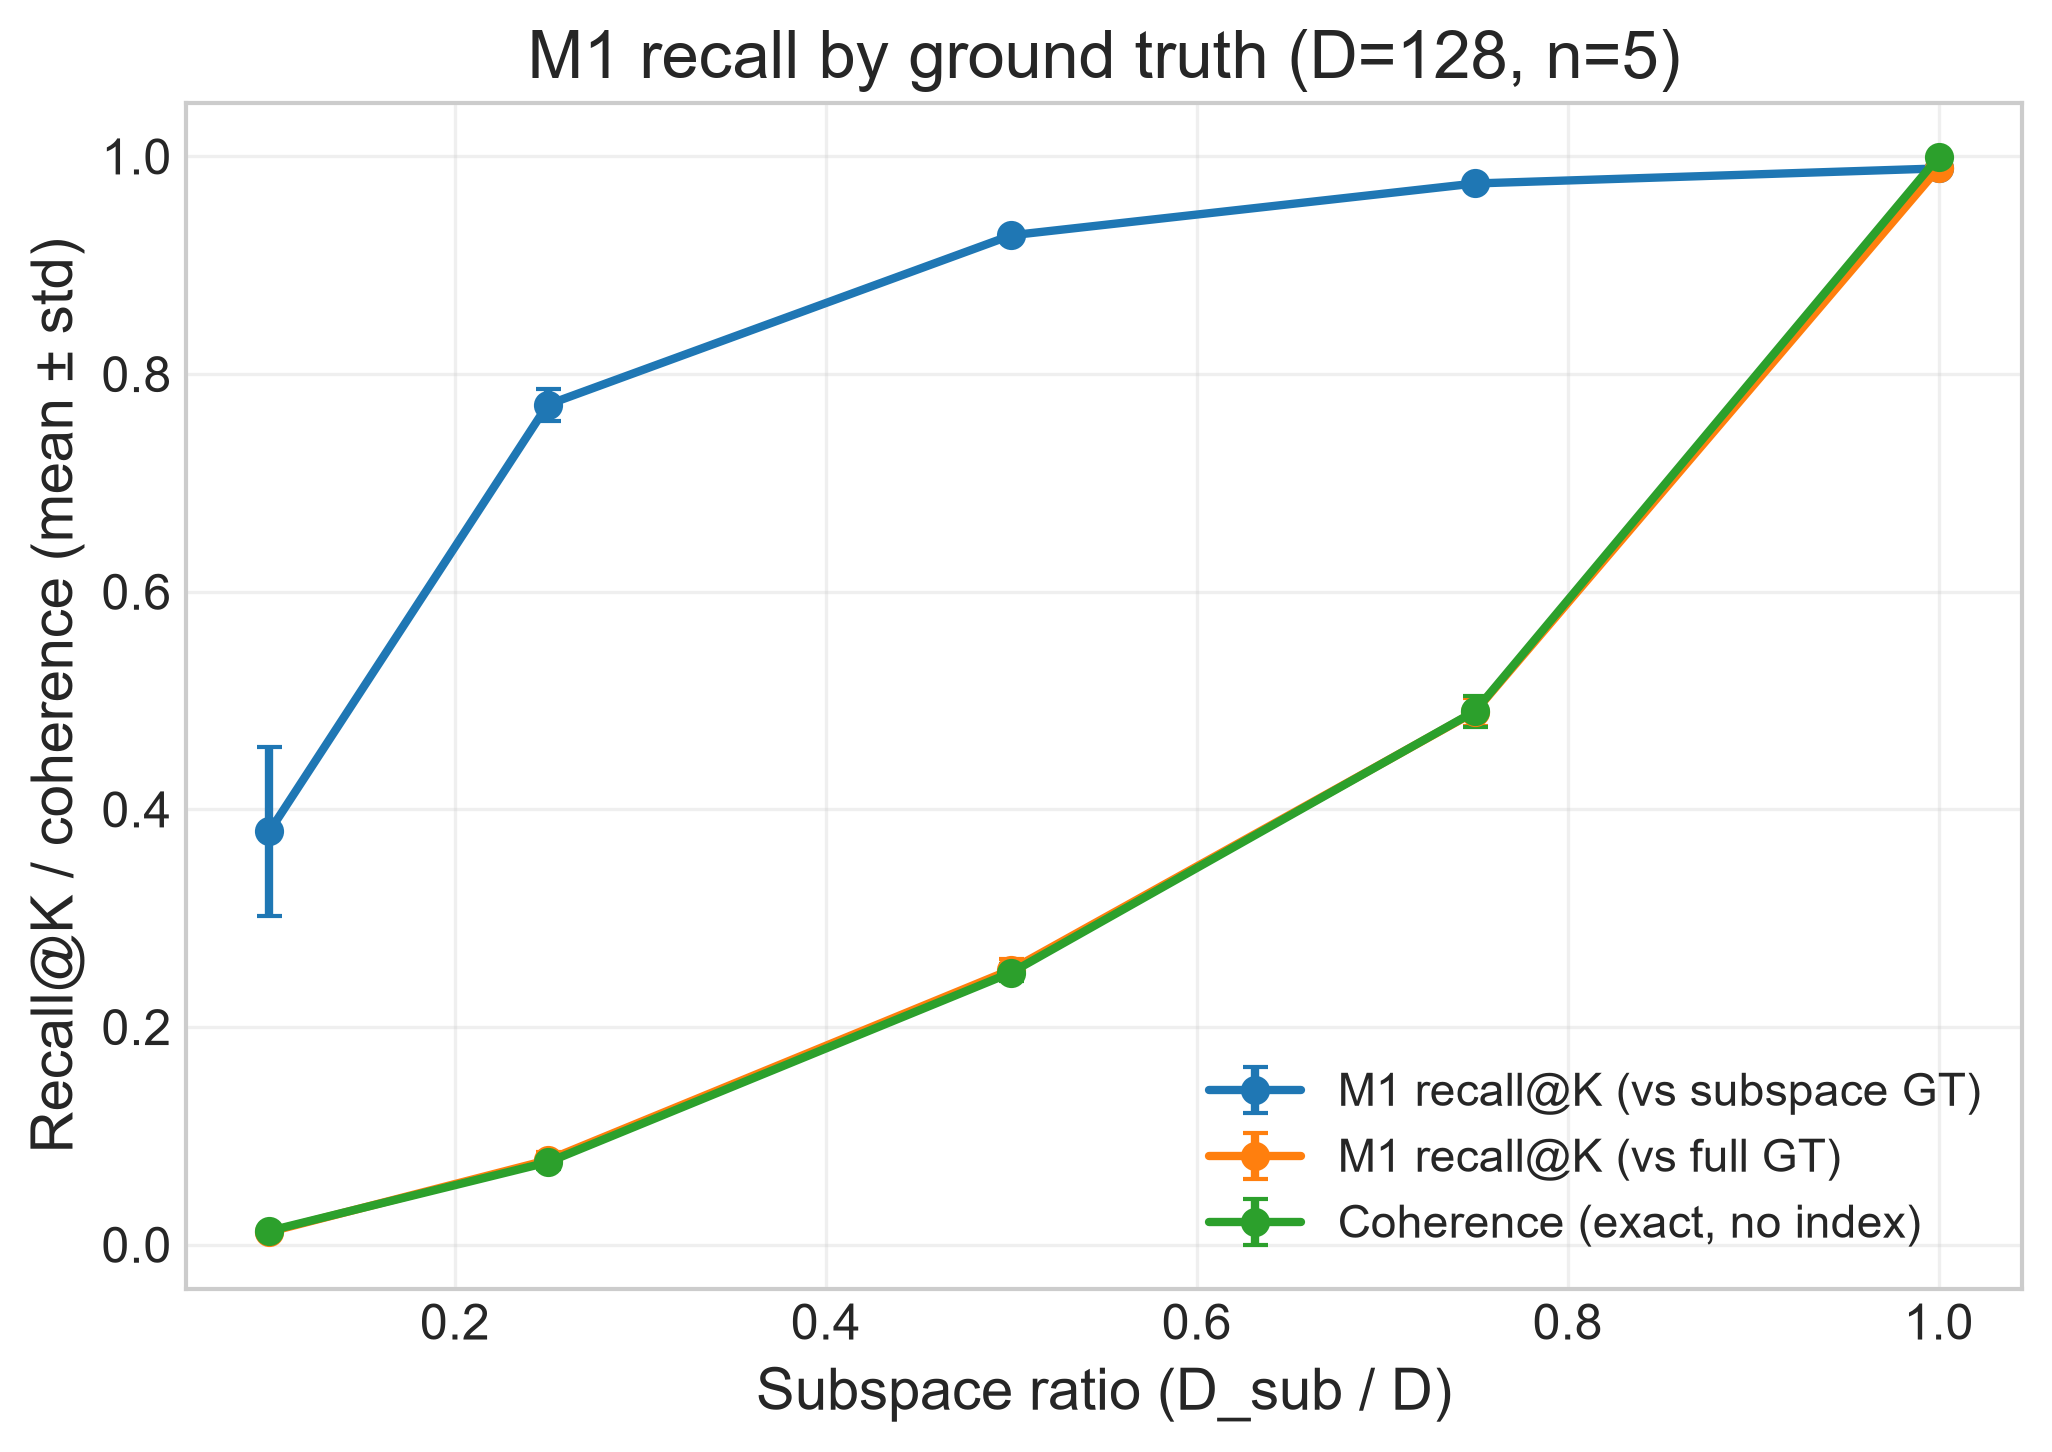
\includegraphics[width=0.92\linewidth]{fig_m1_sift_gt.png}
  \caption{M1 on SIFT1M: Recall@10 against subspace and full-space ground
    truth, and exact coherence (no index), vs.\ ratio (mean$\pm$std,
    $T{=}5$). The full-space curve lies on the coherence curve.}
  \label{fig:m1}
\end{figure}

\subsection{M2: The Cutoff Barely Matters}
\label{sec:eval-m2}

Does keeping full-distance routing on the upper layers recover the subspace
neighbors that M1 misses? Table~\ref{tab:m2} compares cutoffs on the same
SIFT1M index. It barely matters: $L{=}6$ reproduces M1 exactly, cutoffs
$L{=}2$--$4$ gain $0.04$ at ratio $0.1$ ($0.42$ vs.\ $0.38$, within the
across-trial spread), and no cutoff gains more than $0.01$ at larger ratios.
Masking only the base layer ($L{=}1$) already loses as much as masking every
layer, so the loss arises where both designs mask: the base-layer search under
the focus metric. A larger \texttt{ef} for masked queries is the natural
remedy, which we did not sweep.

The synthetic $D{=}768$ corpus cannot inform this question. Plain full-space
search on it reaches only $0.19$ Recall@10 at \texttt{ef}${=}128$, and masked
search reaches $0.21$ subspace recall for every $L\geq 1$ and every ratio we
tested ($0.25$--$0.75$): masking costs nothing there because the index is
already lost without it. Its coherence is also lower than SIFT's ($0.006$ at
ratio $0.1$ to $0.30$ at $0.75$).

\begin{table}[htbp]
  \centering
  \caption{Subspace Recall@10 on SIFT1M by cutoff, one index, $T{=}5$.
    Across-trial std is $\le 0.02$, except $0.05$--$0.08$ at ratio $0.1$.}
  \label{tab:m2}
  \small
  \begin{tabular}{@{}lccc@{}}
    \hline
    \textbf{Design} & \textbf{ratio 0.1} & \textbf{0.25} & \textbf{0.5} \\
    \hline
    M1 (all layers masked) & 0.38 & 0.77 & 0.93 \\
    M2, $L{=}1$ & 0.42 & 0.77 & 0.91 \\
    M2, $L{=}2$--$4$ & 0.42 & 0.78 & 0.93 \\
    M2, $L{=}5$ & 0.40 & 0.77 & 0.93 \\
    M2, $L{=}6$ & 0.38 & 0.77 & 0.93 \\
    \hline
  \end{tabular}
\end{table}

\subsection{Latency: Per-Distance Cost Rules Out a Win}
\label{sec:eval-latency}

No masked configuration beats plain search (Table~\ref{tab:latency}).
In-engine, masked search runs at $0.85$--$0.89\times$ the speed of plain
search at ratio $0.25$ and at $0.70$--$0.75\times$ at ratio $0.75$, so it gets
slower as the focus set grows. A masked request with $L{=}0$ runs at full
speed, so the request path itself adds nothing. With every dimension in focus
(ratio $1.0$), masked search returns the same result set as plain search for
all 500 queries, so it traverses the same nodes, yet it takes $1.94$\,ms
instead of $1.23$\,ms (M1; $1.84$\,ms at $L{=}1$). The gap is therefore
per-distance cost: gathering coordinates from non-contiguous positions is
slower than one contiguous SIMD pass over the full vector, and shrinking the
focus set to a quarter of the dimensions does not make up the difference.
Choosing gather over repack helps in isolation, by $1.24\times$, $1.14\times$,
$1.42\times$, and $1.77\times$ at $D_{\mathrm{sub}}\in\{32,128,384,768\}$
(Figure~\ref{fig:kernel}), but cannot close this gap. For masking to pay off,
a masked distance must cost less than a full contiguous one, for example by
laying registered focus dimensions out contiguously or by approximating
distance comparisons~\cite{gao2023adsampling,chen2023finger,gao2024rabitq}.

\begin{table}[htbp]
  \centering
  \caption{In-engine latency on SIFT1M (host~B): server-side p50 in ms over
    500 queries (best of 3 per query) and speed relative to plain search.}
  \label{tab:latency}
  \small
  \begin{tabular}{@{}lcc@{}}
    \hline
    \textbf{Query} & \textbf{ratio 0.25} & \textbf{ratio 0.75} \\
    \hline
    Plain full search & 1.25 (1.00$\times$) & 1.25 (1.00$\times$) \\
    Focus rescoring (unmasked) & 1.56 (0.80$\times$) & 1.53 (0.81$\times$) \\
    Masked, $L{=}0$ & 1.25 (1.00$\times$) & 1.23 (1.02$\times$) \\
    M2, $L{=}1$ & 1.46 (0.85$\times$) & 1.79 (0.70$\times$) \\
    M2, $L{=}3$ & 1.41 (0.89$\times$) & 1.67 (0.75$\times$) \\
    M1 & 1.44 (0.87$\times$) & 1.69 (0.74$\times$) \\
    V1, $L{=}1$, $m{=}8$ & 1.73 (0.72$\times$) & 1.95 (0.64$\times$) \\
    \hline
  \end{tabular}
\end{table}

\begin{figure}[htbp]
  \centering
  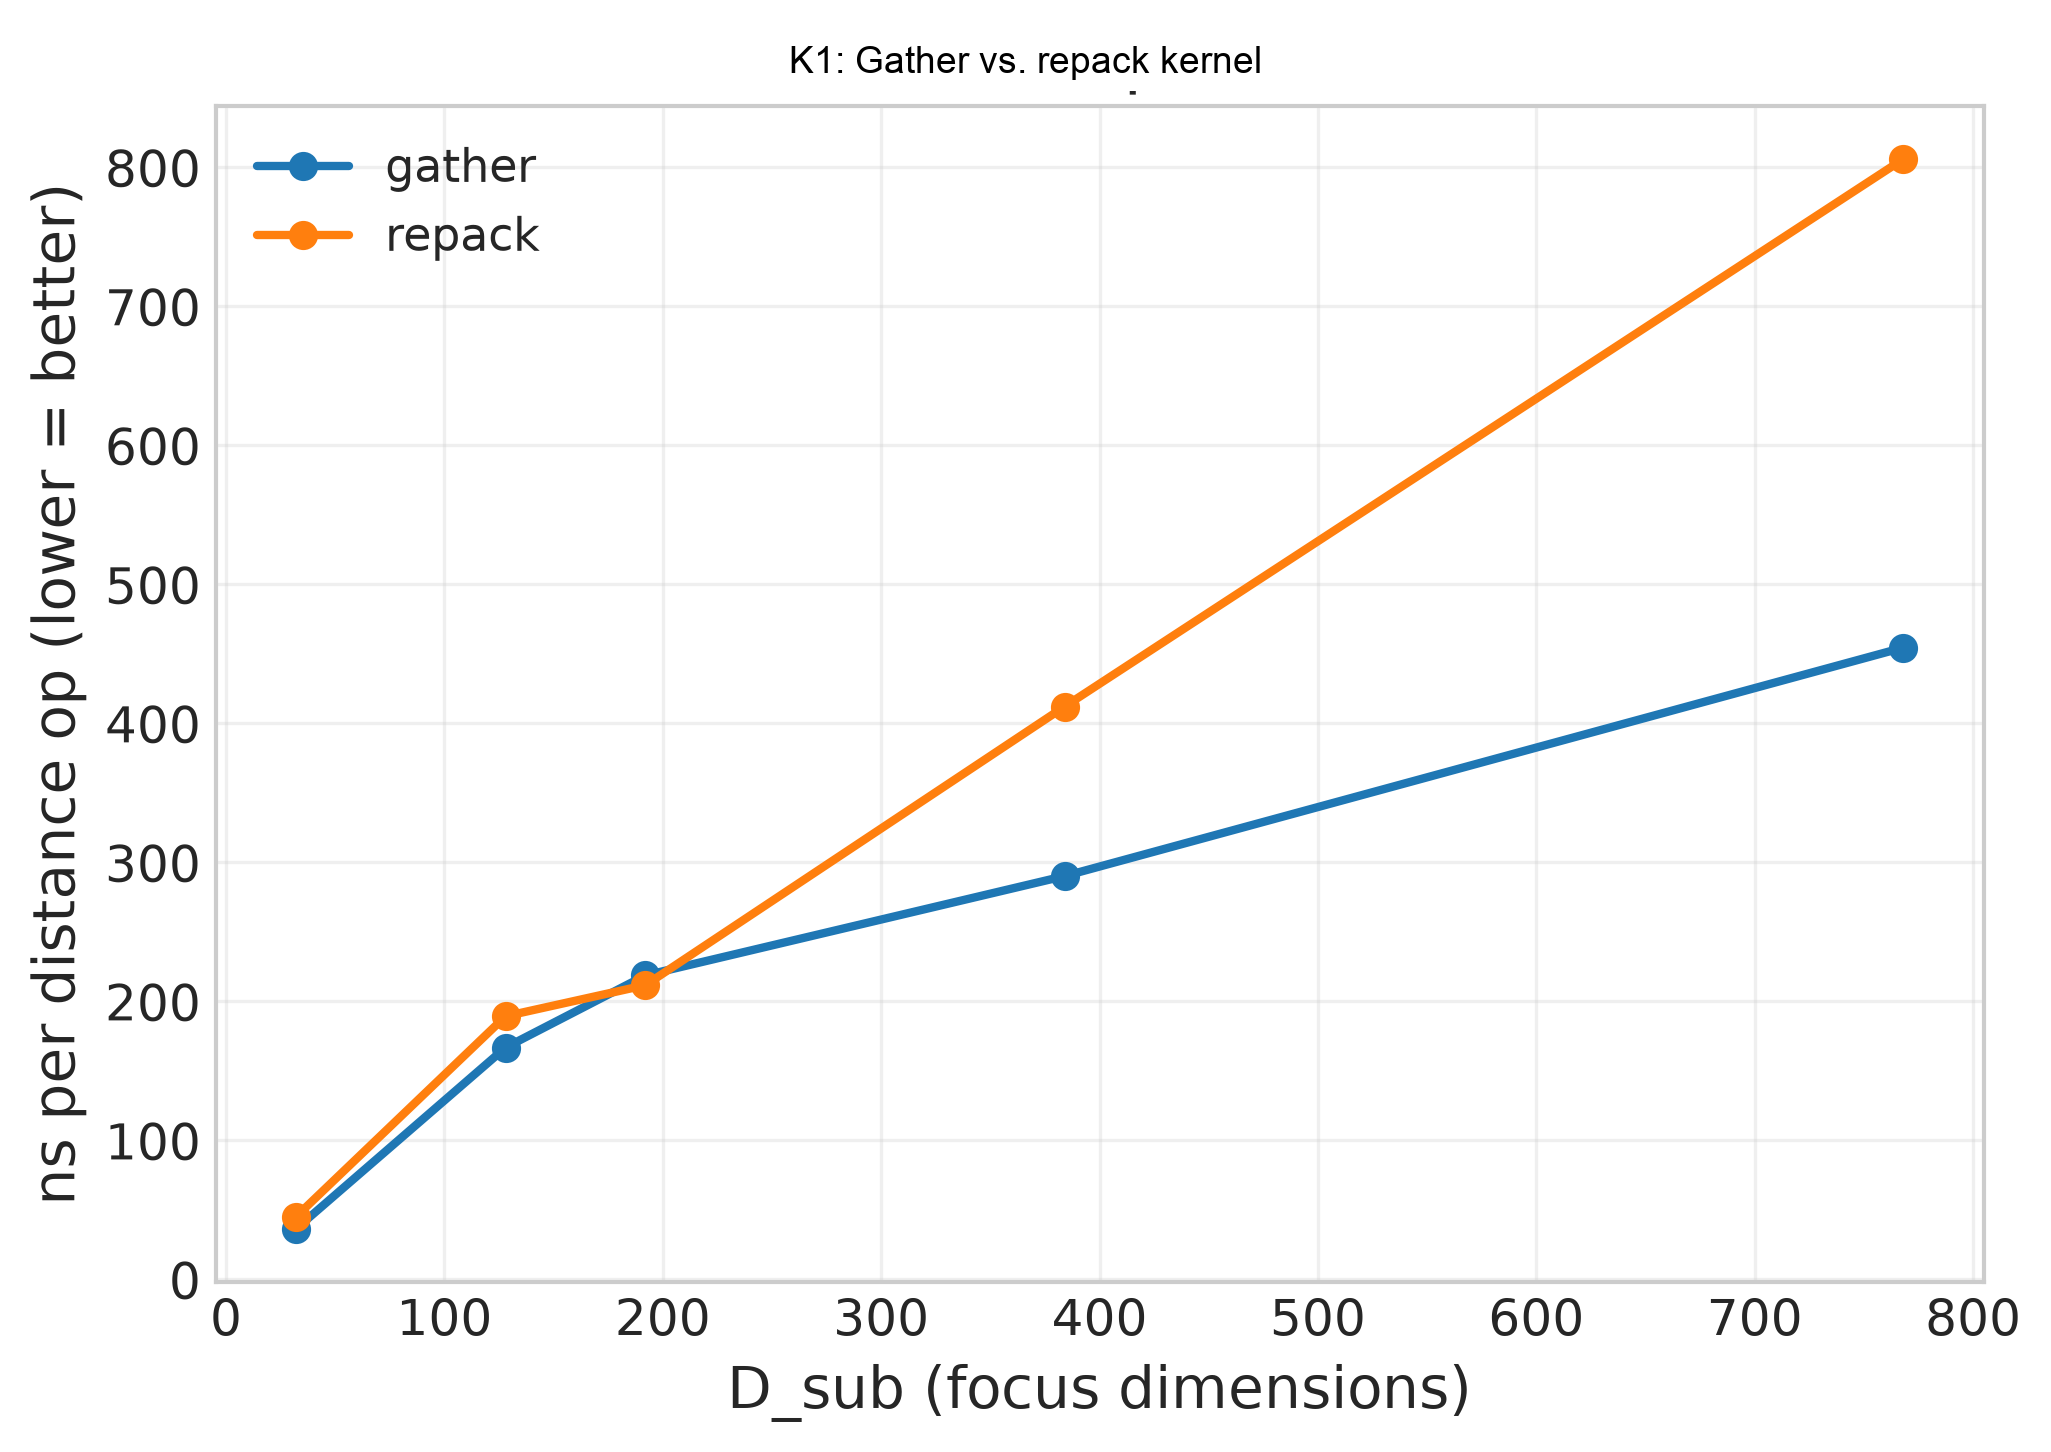
\includegraphics[width=0.92\linewidth]{fig_xcut1_kernels.png}
  \caption{K1: Masked Dot-product kernel cost, repack vs.\ gather (ns/op,
    host~A).}
  \label{fig:kernel}
\end{figure}

\subsection{V1: Verify + Overfetch Recovers Recall Where Coherence Allows}
\label{sec:eval-verify}

Since masked search returns subspace neighbors, can a post-traversal
full-distance pass recover the full-space ones? At overfetch $m{=}1$, masked
and verified Recall@10 are identical, as predicted in
Section~\ref{sec:masked}. At $m{=}8$ on SIFT1M with $L{=}1$, full-space
recall rises well above the coherence level, from $0.24$ to $0.61$ at ratio
$0.5$ and from $0.48$ to $0.91$ at ratio $0.75$ (Figure~\ref{fig:verify});
with every layer masked the results are similar ($0.64$ and $0.93$). The
candidate pool is now the top-$80$ under the focus metric, and verification
recovers whatever part of the full-space top-$10$ it contains; at ratio $0.1$
that part is small ($0.01\rightarrow 0.06$). In-engine, overfetching and
verifying add $0.16$--$0.26$\,ms (Table~\ref{tab:latency}), of which the
rescore itself is at most $0.12$\,ms.

\begin{figure}[htbp]
  \centering
  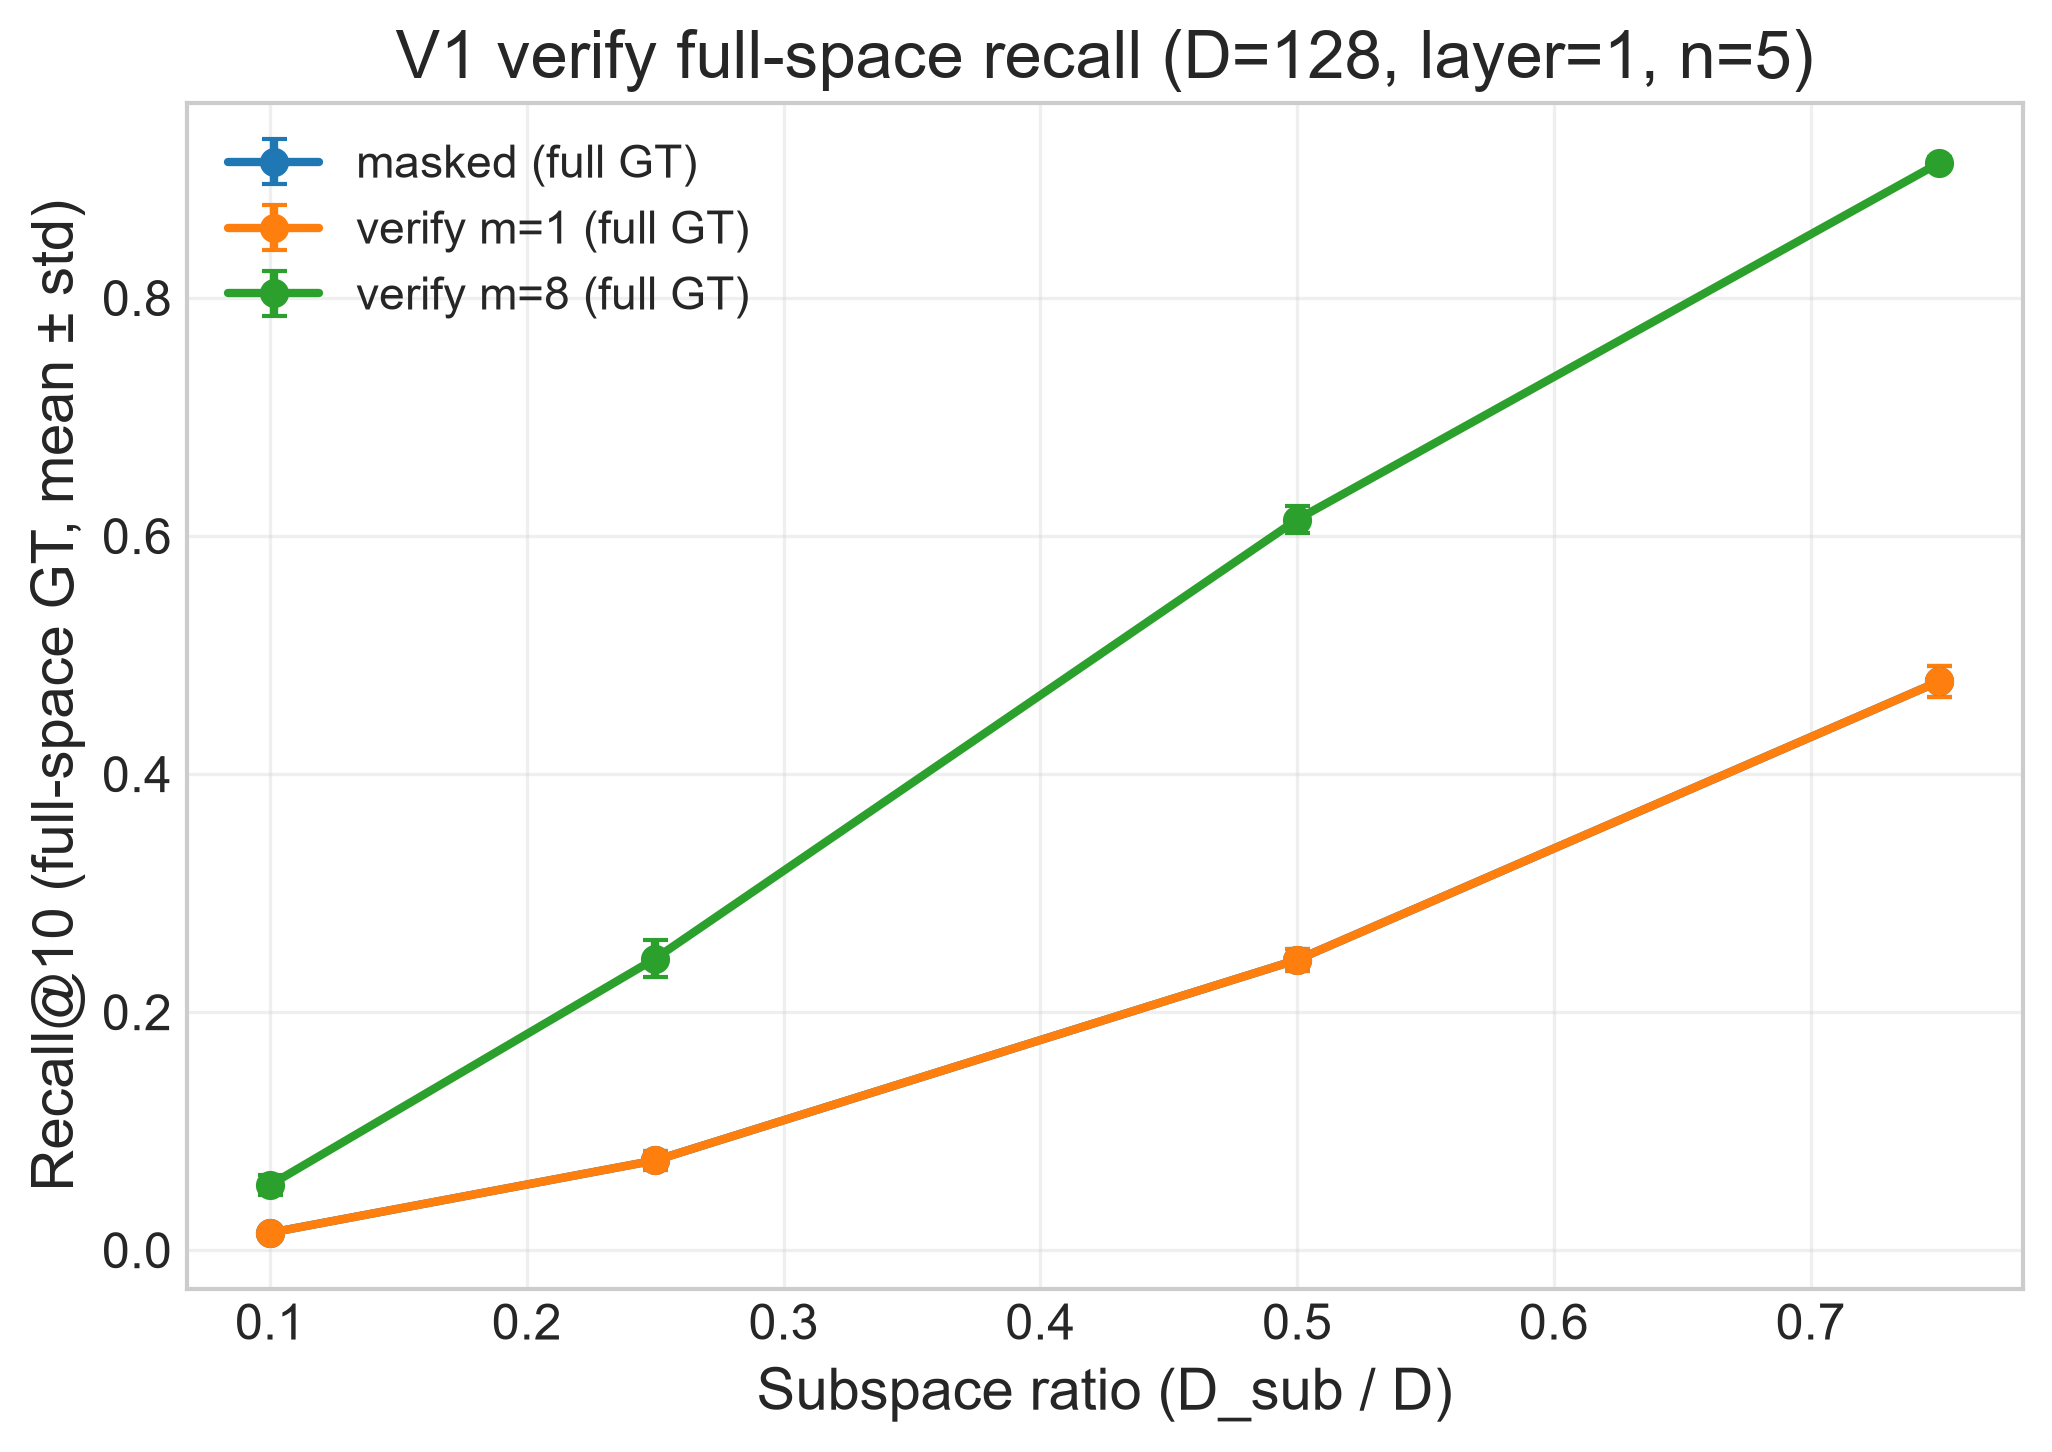
\includegraphics[width=0.92\linewidth]{fig_xcut3_sift_full.png}
  \caption{V1 on SIFT1M with $L{=}1$: full-space Recall@10 without
    verification, with verification at $m{=}1$, and at $m{=}8$
    (mean$\pm$std, $T{=}5$). The unverified curve is hidden under $m{=}1$,
    which returns the same set by construction.}
  \label{fig:verify}
\end{figure}

\subsection{M3: Blending Never Beats Pure Masking}
\label{sec:eval-m3}

Finally, we test whether M3's continuous $\alpha$ can improve on M2.
Figure~\ref{fig:m3} shows that on SIFT1M at ratio $0.25$, subspace recall is
highest at $\alpha{=}0$ for every cutoff ($0.77$ at $L{=}1$ and $0.78$ at
$L{=}2$, matching Table~\ref{tab:m2}) and falls monotonically to the $L{=}0$
(coherence) level of $0.075$ as $\alpha\rightarrow 1$; already at
$\alpha{=}0.25$ it drops to $0.21$. Since $\alpha{=}0$ is exactly M2,
blending adds API surface and computes both distances without ever improving
on the simpler design; we do not recommend shipping M3.

\begin{figure}[htbp]
  \centering
  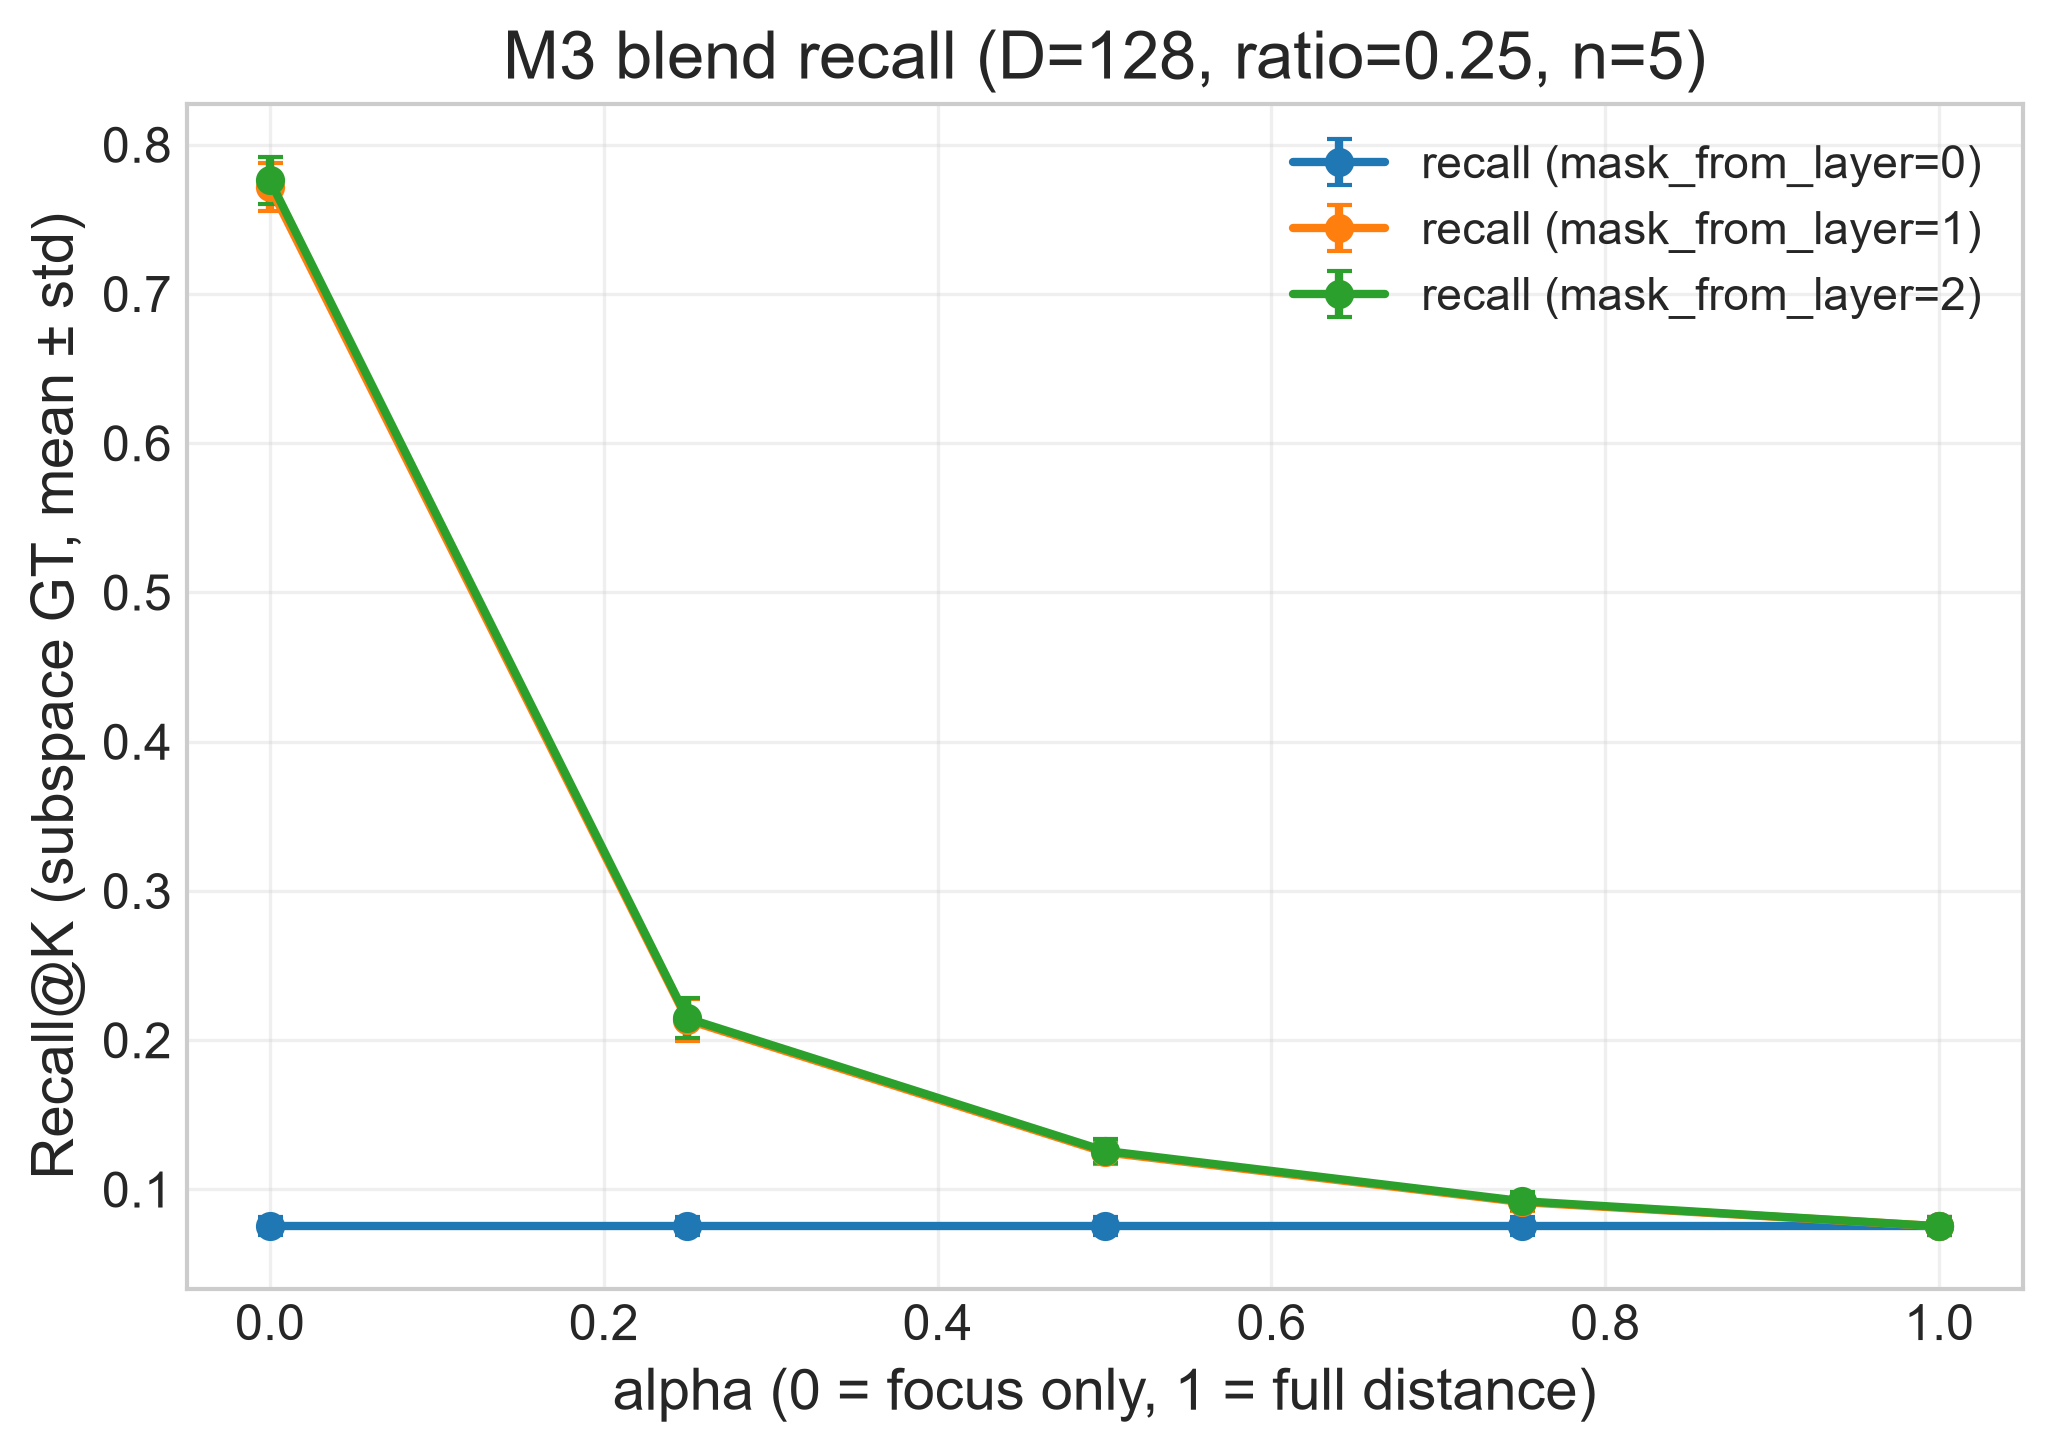
\includegraphics[width=0.92\linewidth]{fig_option4_sift.png}
  \caption{M3 on SIFT1M: subspace Recall@10 vs.\ $\alpha$ for cutoffs
    $\{0,1,2\}$ at ratio $0.25$ (mean$\pm$std, $T{=}5$).}
  \label{fig:m3}
\end{figure}

\subsection{Summary}

Table~\ref{tab:keep} consolidates the verdict for each mechanism.

\begin{table}[htbp]
  \centering
  \caption{Verdict per mechanism.}
  \label{tab:keep}
  \footnotesize
  \setlength{\tabcolsep}{3pt}
  \begin{tabular}{@{}>{\raggedright\arraybackslash}p{0.28\columnwidth}
                     >{\raggedright\arraybackslash}p{0.18\columnwidth}
                     >{\raggedright\arraybackslash}p{0.46\columnwidth}@{}}
    \hline
    \textbf{Mechanism} & \textbf{Verdict} & \textbf{Evidence} \\
    \hline
    Attribution (in-DB) & Keep & $+$0.4\,ms in-engine; $\sim$1.8$\times$ vs.\ post-query \\
    Focus rescoring only & Not accel. & 0.80$\times$ plain speed (\S\ref{sec:eval-attr}) \\
    M1 all-layer mask & Keep & Full-space recall $=$ coherence; subspace recall 0.38--0.98 (\S\ref{sec:eval-gt}) \\
    M2 hybrid cutoff & Optional & At most $+$0.04 subspace recall over M1 (\S\ref{sec:eval-m2}) \\
    K1 gather kernel & Keep (micro) & 1.1--1.8$\times$ vs.\ repack; masked still slower than plain (\S\ref{sec:eval-latency}) \\
    C1 coherence & Keep & Equals full-space recall of masked search \\
    V1, $m{=}1$ & API only & Recall@$k$ provably unchanged \\
    V1 + overfetch & Keep & Recovers full-space recall where coherence allows; $+$0.2\,ms \\
    M3 blend & Skip & Best at $\alpha{=}0$, i.e.\ M2 \\
    \hline
  \end{tabular}
\end{table}

%=============================================================================
\section{Related Work}
\label{sec:related}

\paragraph{Vector databases.} Milvus~\cite{wang2021milvus},
Pinecone~\cite{pinecone2023}, and Qdrant~\cite{qdrant2024} expose ANN with
filters and quantization; AnalyticDB-V~\cite{wei2020analyticdbv} and
PASE~\cite{yang2020pase} bring ANN indexes into relational engines, and VBase~\cite{zhang2023vbase} unifies vector search with
relational operators. Pan et al.~\cite{pan2024survey} survey the design
space. None exposes per-coordinate score decompositions or layer-aware masked
metrics. We add in-database attribution and query-time masked HNSW scoring
inside an existing production graph index.

\paragraph{ANN search.} FAISS~\cite{johnson2019faiss} and
ScaNN~\cite{guo2020scann} optimize large-scale search, and experimental
studies compare ANN methods under common
protocols~\cite{wang2021graphsurvey,aumuller2020annbench,echihabi2019hydra};
explainability and dynamic subspace routing remain outside the index.
ADSampling~\cite{gao2023adsampling}, FINGER~\cite{chen2023finger}, and
RaBitQ~\cite{gao2024rabitq} speed up search by making distance comparisons
cheaper; our latency results (Section~\ref{sec:eval-latency}) suggest masked
search needs comparably cheap comparisons to pay off.

\paragraph{Subspace and constrained search.} $k$-NN queries over arbitrary
query-time subspaces have been studied with dedicated index
structures~\cite{lian2008subspace,bernecker2010subspace}, and
MUST~\cite{wang2024must} searches concatenated multimodal vectors under
learned per-modality weights, of which a modality mask is a special case.
Filtered graph
search faces a related problem: when a predicate changes which points
qualify, a graph built for the unconstrained query can lose navigability,
which ACORN~\cite{patel2024acorn} and
Filtered-DiskANN~\cite{gollapudi2023filtered} address by changing graph
construction. We instead measure what an unmodified full-space HNSW graph
delivers under a query-time masked metric.

\paragraph{Explaining query answers.} Database work explains query results
through causality and intervention over input
tuples~\cite{meliou2010causality,roy2014explanations}. A similarity score is
instead a sum of per-coordinate terms, the aggregate-of-grades score model of
top-$k$ processing~\cite{fagin2003optimal}, so explaining it needs no search
over inputs: attribution reports each coordinate's exact share of the score,
as an OLAP roll-up reports each group's share of a total~\cite{gray1998data}.
Model explainers such as SHAP and LIME~\cite{lundberg2017shap,ribeiro2016lime}
estimate attributions by sampling or local surrogates instead.

\paragraph{Dimension reduction and projected indexes.} Static projections or
multi-index layouts differ from \emph{query-time} focus sets evaluated against
an existing full-dimensional HNSW index. A dedicated auxiliary index per focus
set would avoid both the recall loss for small focus sets
(Section~\ref{sec:eval-m2}) and the gather cost
(Section~\ref{sec:eval-latency}), but only for a registered palette of
subspaces; we leave it to future work (Section~\ref{sec:discussion}).

%=============================================================================
\section{Discussion and Conclusion}
\label{sec:discussion}

\paragraph{Shipping verdict.} Keep in-database attribution. Keep masked
traversal as a semantics feature for subspace search, with V1 overfetch when
callers need full-space neighbors; the layer cutoff can stay as an optional
knob, and M3 should go. In this implementation masked traversal is not a
speed feature.

\paragraph{Latency.} Masking lost to plain search in every configuration
because a gathered distance costs more than a contiguous one
(Section~\ref{sec:eval-latency}). Laying registered focus sets out
contiguously, or a dedicated projected index per registered focus set
(Section~\ref{sec:related}), are the natural next steps.

\paragraph{Limitations.} SIFT1M is our only corpus on which plain HNSW
search is accurate; on the i.i.d.\ synthetic corpus plain search reaches only
$0.19$ Recall@10, and real encoder embeddings remain to be tested. We did not
sweep \texttt{ef} for masked queries, and each masked-traversal result comes
from a single index per corpus.

XQdrant shows exact feature attribution can live in a Rust vector engine at a
small in-engine cost and a clear end-to-end win over client-side extraction.
For masked-distance HNSW, the main lesson is methodological: recall must be
measured against the right ground truth. Against full-space ground truth,
masked traversal of a full-space graph scores the subspace/full-space
coherence, a property of the data rather than of the index; against subspace
ground truth, it navigates well for large focus sets and degrades for small
ones. It never beats plain search, because each masked distance costs more
than a full contiguous one. The public experiment index
(Section~\ref{sec:artifacts}) maps each claim to a reproducible run.

%=============================================================================
%% EDBT: required section name "Artifacts"; does NOT count toward the 6-page limit.
\section{Artifacts}
\label{sec:artifacts}

Source code (XQdrant fork of Qdrant) and the experiment harness are public:
\begin{itemize}
  \setlength{\itemsep}{0.15em}
  \setlength{\parsep}{0pt}
  \item Engine fork at the evaluated commit:
    \url{https://github.com/Moetez-Fradi/XQdrant/tree/ed5ca79}
  \item Experiment index and scripts\pending{, plus canonical CSVs}:
    \url{https://github.com/Moetez-Fradi/XAI/tree/main/DB_systems}
\end{itemize}
The harness contains the unified orchestration script, per-mechanism runners,
plotting entry points for M1--M3, K1, C1, and V1, and build/run notes for the
XQdrant binary and the vanilla Qdrant baseline. Neither repository uses access
monitoring.

\bibliographystyle{ACM-Reference-Format}
\bibliography{main}

\end{document}
